\chapter{Grupos de homología relativa}
\section{Qué aporta un subespacio a la homología}
Como vimos en el tema anterior, el grupo de homología de orden 1 de la rosa tiene tantos generadores como pétalos. De hecho, para ser más exactos, podemos hallar un representante de cada generador en uno de los pétalos.

\begin{figure}[h]
\centering
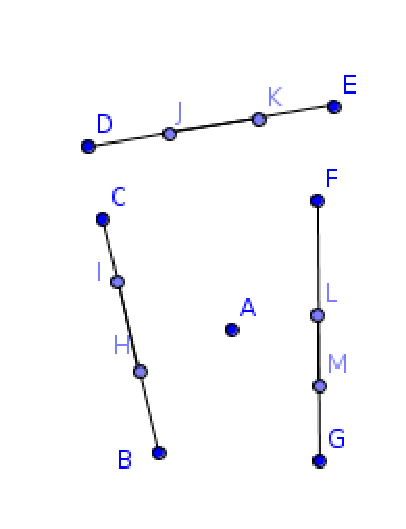
\includegraphics[scale=0.75]{Figures/Gen3Rosa.eps}
\caption{Representación de la rosa de 3 pétalos. Los segmentos $[I,H]$, $[J,K]$ y $[L,M]$ son los generadores de $H_1(B_3)$.}
\end{figure}

Esto parece decirnos que la acción de \textbf{añadir un pétalo} (que se llama \textbf{pegamento} o \textbf{adjunción}, como veremos en el capítulo siguiente) es la que provoca la aparición de nuevos generadores. No obstante, diferentes adjunciones provocan diferentes alteraciones:

\begin{enumerate}
\item Si pegamos sólo uno de los extremos del segmento a $B_p$ y dejamos el otro libre, $B_p$ es un retracto por deformación fuerte de la figura resultante, de forma que no aparecen nuevos generadores.
\item Si lo pegamos por ambos lados, aparece un pétalo nuevo y aparece un nuevo generador.
\end{enumerate}


Dado un espacio topológico $X$ y un subespacio $A \subseteq X$, el grupo de homología relativa estudia cómo $A$ está pegado con su complementario, $X-A$. Diremos que dos cadenas son \textit{iguales módulo $A$} si su diferencia es una cadena en $A$. En particular, tendremos que una cadena será un \textit{ciclo módulo $A$} si su borde está contenido en $A$.

\section{Complejo de cadenas cociente}
Diremos que un complejo de cadenas $(D,\partial')$ es un \textbf{subcomplejo} de $(C,\partial)$ si, dado un $p \in \mb{Z}$, se verifica que $$D_p \leq C_p \quad \land \quad \partial_p(D_p)\subseteq D_{p-1}$$

Un subcomplejo $(D,\partial)$ es \textbf{subcomplejo normal} de $(C,\partial)$ si $D$ es un subgrupo graduado normal de $C$.

\cuadro{Sea $(C,\partial)$ un complejo de cadenas y $(D,\partial')$ un subcomplejo de cadenas tal que $D \trianglelefteq C$. Se define el \textbf{complejo cociente} como el graduado $C/D$ dotado del operador borde siguiente: $$\funcio{Q_p}{C_p/D_p}{C_{p-1}/D_{p-1}}{c+D_p}{(\partial_p c)+D_{p-1}}$$}

Si $\pi: C \longrightarrow C/D$ es el epimorfismo canónico e $i: D \hookrightarrow C$ es la inclusión, se tiene que la sucesión $$0 \longrightarrow D \xrightarrow{i} C \xrightarrow{\pi} \frac{C}{D} \longrightarrow 0$$ es exacta. Según el teorema \ref{SucExacHomo}, si podemos hallar un homomorfismo de conexión $\Delta: H_*(C/D) \longrightarrow H_*(C)$ de grado -1, \ecua{\label{SECociente}H_n(D) \xrightarrow{i_*} H_n(C) \xrightarrow{\pi_*} H_n\left(\frac{C}{D}\right) \xrightarrow{\Delta} H_{n-1}(D)} será una sucesión exacta larga.
\\

\begin{nota}
Por cuestiones de economía en la notación, a la clase del elemento $c \in C_p$ en el grupo cociente $H_p(C/D)$ se la denotará como $[c+D_p]$ o simplemente $\la c\ra$. De esta forma, se reserva $[c]$ para la clase de $c$ en $H_*(C)$.
\end{nota}

Para construir el homomorfismo de conexión, sea $[c] \in Z_n(C/D)$. Se tiene que $$\partial_n c+D_n=0+D_{n-1} \implies \partial c \in D_{n-1}$$ Como $\partial(\partial c)=\partial^2c=0$, $\partial c \in Z_{n-1}(D)$, luego $\partial c+B_{n-1}(D) \in H_{n-1}(D)$. Definimos entonces el homomorfismo \ecua{\label{DeltaCociente}\funcio{\Delta_n}{H_n(C/D)}{H_{n-1}(D)}{c+D_n}{\partial c + B_{n-1}(D)}} de forma que $\Delta=\{\Delta_n: n \in \mb{Z}\}$ es un homomorfismo de conexión, haciendo que (\ref{SECociente}) sea una sucesión exacta larga.

\begin{lema}[Teorema de isomorfia para grupos graduados]\label{TTIGG}
Sea $C$ un complejo de cadenas y $E,D$ subcomplejos normales de $C$. Si $E$ es un subcomplejo de $D$, $$\frac{C}{D} \cong \frac{C/E}{D/E}$$
\end{lema}

\begin{proof}
Sea $p \in \mb{Z}$. Por definición de subcomplejo y subcomplejo normal, $D_p,E_p \trianglelefteq C_p$ y $E_p \leq D_p$. Por el tercer teorema de isomorfia, existe un isomorfismo $$f_p: \frac{C_p}{D_p} \longrightarrow \frac{C_p/E_p}{D_p/E_p}$$

Considérese entonces el homomorfismo graduado $f=\underset{p \in \mb{Z}}{\{f_p\}}$. Se tiene que $$f: \frac{C}{D} \longrightarrow \frac{C/E}{D/E}$$ es un isomorfismo graduado por ser una colección de isomorfismos. Por tanto, $C/D$ es isomorfo a $(C/E)/(D/E)$.
\end{proof}

Sea $C$ un complejo de cadenas y $E \leq D$ subcomplejos normales de $C$. Por el lema \ref{TTIGG}, existe un isomorfismo graduado $f: (C/E)/(D/E) \longrightarrow C/D$. Si ahora consideramos el epimorfismo canónico $\pi: C/E \longrightarrow (C/E)/(D/E)$, se tiene que $$\Pi: \frac{C}{E} \xrightarrow{\pi} \frac{C/E}{D/E} \xrightarrow{f} \frac{C}{D}$$ es un epimorfismo graduado entre $C/E$ y $C/D$. De aquí se obtiene la sucesión exacta corta $$0 \longrightarrow \frac{D}{E} \xrightarrow{i} \frac{C}{E} \xrightarrow{\Pi}\frac{C}{D} \longrightarrow 0$$

Dado un $n \in \mb{Z}$, sea $p_n: D_n \longrightarrow D_n/E_n$ el epimorfismo canónico. Se tiene que $p=\{p_n: n \in \mb{Z}\}$ induce un homomorfismo de grado 0 en homología, $$p_*: H_*(D) \longrightarrow H_*(D/E)$$ Si $\Delta: H_*(C/D) \longrightarrow H_*(D)$ es el homomorfismo graduado (\ref{DeltaCociente}), \ecua{\label{DeltaCPrima}\Delta': H_*(C/D) \xrightarrow{\Delta} H_*(D) \xrightarrow{p_*} H_*(D/E)} es un homomorfismo de conexión, por lo que el teorema \ref{SucExacHomo} nos dice que \ecua{\label{SECociente2}H_n\left(\frac{D}{E}\right) \xrightarrow{i_*}H_n\left(\frac{C}{E}\right)\xrightarrow{\Pi_*}H_n\left(\frac{C}{D}\right)\xrightarrow{\Delta'}H_{n-1}\left(\frac{D}{E}\right)} es una sucesión exacta larga.
\\

Sea $C'$ otro complejo de cadenas, con $E'\leq D'$ subcomplejos normales de $C'$. Considérese una aplicación de cadenas $g: C \longrightarrow C'$ tal que $g(D) \leq D'$ y $g(E) \leq E'$. Como acabamos de ver, se puede construir una sucesión exacta corta $$0 \longrightarrow \frac{D'}{E'} \longrightarrow \frac{C'}{E'} \longrightarrow \frac{C'}{D'} \longrightarrow 0$$ que induce una sucesión exacta larga en homología similar a (\ref{SECociente2}). Dado que $g$ es una aplicación de cadenas, podemos conectar ambas sucesiones exactas usando $g_*$: \ecua{\label{TNatural}\begin{array}{ccccccc}
H_n\left(\frac{D}{E}\right)&\xrightarrow{i_*}&H_n\left(\frac{C}{E}\right)&\xrightarrow{\Pi_*}&H_n\left(\frac{C}{D}\right)&\xrightarrow{\Delta'}&H_{n-1}\left(\frac{D}{E}\right)\\
%&&&&&&\\
g_*\downarrow&\circlearrowleft&g_*\downarrow&\circlearrowleft&g_*\downarrow&\circlearrowleft&g_*\downarrow\\
%&&&&&&\\
H_n\left(\frac{D'}{E'}\right)&\xrightarrow{\tilde{i}_*}&H_n\left(\frac{C'}{E'}\right)&\xrightarrow{\tilde{\Pi}_*}&H_n\left(\frac{C'}{D'}\right)&\xrightarrow{\tilde{\Delta}'}&H_{n-1}\left(\frac{D'}{E'}\right)
\end{array}}

Por cómo está construida la sucesión exacta (\ref{SECociente2}), se puede probar que cada uno de los cuadrados del diagrama (\ref{TNatural}) es conmutativo. Es decir, $$g_*\circ \tilde{i}_*=i_*\circ g_*; \quad g_*\circ \tilde{\Pi}_*=\Pi_*\circ g_*; \quad g_*\circ \tilde{\Delta}'=\Delta'\circ g_*$$ Se dice entonces que $g_*$ es una \textbf{transformación natural} o que cumple la \textbf{hipótesis de naturalidad}.
\\

\section{Homología singular relativa}
\cuadro{Un \textbf{par de espacios} es un par ordenado de la forma $(X,A)$, donde $X \in \topo$ y $A \subseteq X$ es un subespacio.}

Sea $(X,A)$ un par de espacios y $n > 0$. Dado un $c \in S_n(X)$, existen $n$-símplices singulares $$\phi_1,\dots,\phi_p: \sigma_n \longrightarrow X$$ y $\mu_1,\dots,\mu_p \in \mb{Z}$ tales que $$c=\sum^p_{i=1}\mu_i\phi_i$$ Si $\phi_i(\sigma_n) \subseteq A$ para cada $i=1,\dots,p$, se tiene entonces que $c \in S_n(A)$. De aquí se sigue que $S_n(A) \leq S_n(X)$.
\\

Por otro lado, dado un $i=0,\dots,n$, $$\partial_{(i)} \phi(\sigma_{n-1}) \subset \phi(\sigma_n) \subset A \implies \partial_{(i)}\phi \in S_{n-1}(A)$$ Dado que $$\partial_n \phi=\sum^n_{i=0}\partial_{(i)}\phi$$ se tiene que $\partial_n \phi \in S_{n-1}(A)$, por lo que $S_*(A)$ dotado del operador borde $\partial_A=\{\partial_n|_{S_n(A)}: n \in \mb{Z}\}$ es un subcomplejo de cadenas de $S_*(X)$.
\\

Se define el \textbf{complejo de cadenas singulares de $X$ módulo $A$} como el complejo cociente $$S_*(X,A):=\frac{S_*(X)}{S_*(A)}=\left\{\frac{S_n(X)}{S_n(A)}: n \in \mb{Z}\right\}$$ De la misma forma, se definen los grupos graduados $$Z_*(X,A):=\frac{Z_*(X)}{Z_*(A)}; \quad B_*(X,A):=\frac{B_*(X)}{B_*(A)}; \quad n \geq 0$$

\noindent\textbf{Una transformación que preserva el orden:}\\
Sean $X,Y$ espacios topológicos. Las relaciones binarias \textit{$X \leq Y$ si y sólo si $X$ es un subespacio topológico de $Y$} y \textit{$S_*(X) \leq S_*(Y)$ si sólo si $S_*(X)$ es un subcomplejo de cadenas de $S_*(X)$} son relaciones de orden, y acabamos de demostrar que $$X \leq Y \implies S_*(X) \leq S_*(Y)$$ Desde un punto de vista informal, podríamos decir que la transformación $X \mapsto S_*(X)$ \textit{preserva el orden}, porque transforma subespacios topológicos en subcomplejos de cadenas.

\cuadro{Sea $(X,A)$ un par de espacios. Se define el \textbf{grupo $n$-ésimo de homología singular relativa de $X$ módulo $A$} como $$H_n(X,A):=H_n(S_*(X,A))=\frac{Z_n(X,A)}{B_n(X,A)}$$}

\begin{ejem}\label{EjEsfera}
Sea $X=S^2$. Considérense las curvas $c,d \subset X$ mostradas en la figura \ref{FigEsfera}, y sea $A$ la componente conexa de $X-d$ que no contiene a la curva $c$.
\\

Usando el ejemplo \ref{CaminoCiclo}, $c$ forma un ciclo en $X$ por ser un lazo, por lo que $\partial_1 c=0$. Por cómo se define el operador borde del complejo de cadenas cociente, $$\partial_1(c+S_1(A))=\partial_1 c+S_1(A)=0+S_1(A)$$ por lo que $c$ forma un ciclo en $(X,A)$.
\\

Sea $e$ el arco de circunferencia que une las curvas $c$ y $d$ en $X$, y $\tilde{A}=A\cup d$. $e$ no es un ciclo en $X$ porque no es un lazo, y tampoco es un ciclo en $(X,\tilde{A})$. No obstante, sí es un ciclo en $(X,\tilde{A}\cup c)$. Notar que ambos extremos del camino $e$ caen en algún punto de $\tilde{A}\cup c$.
\end{ejem}

\begin{figure}[h]
\centering
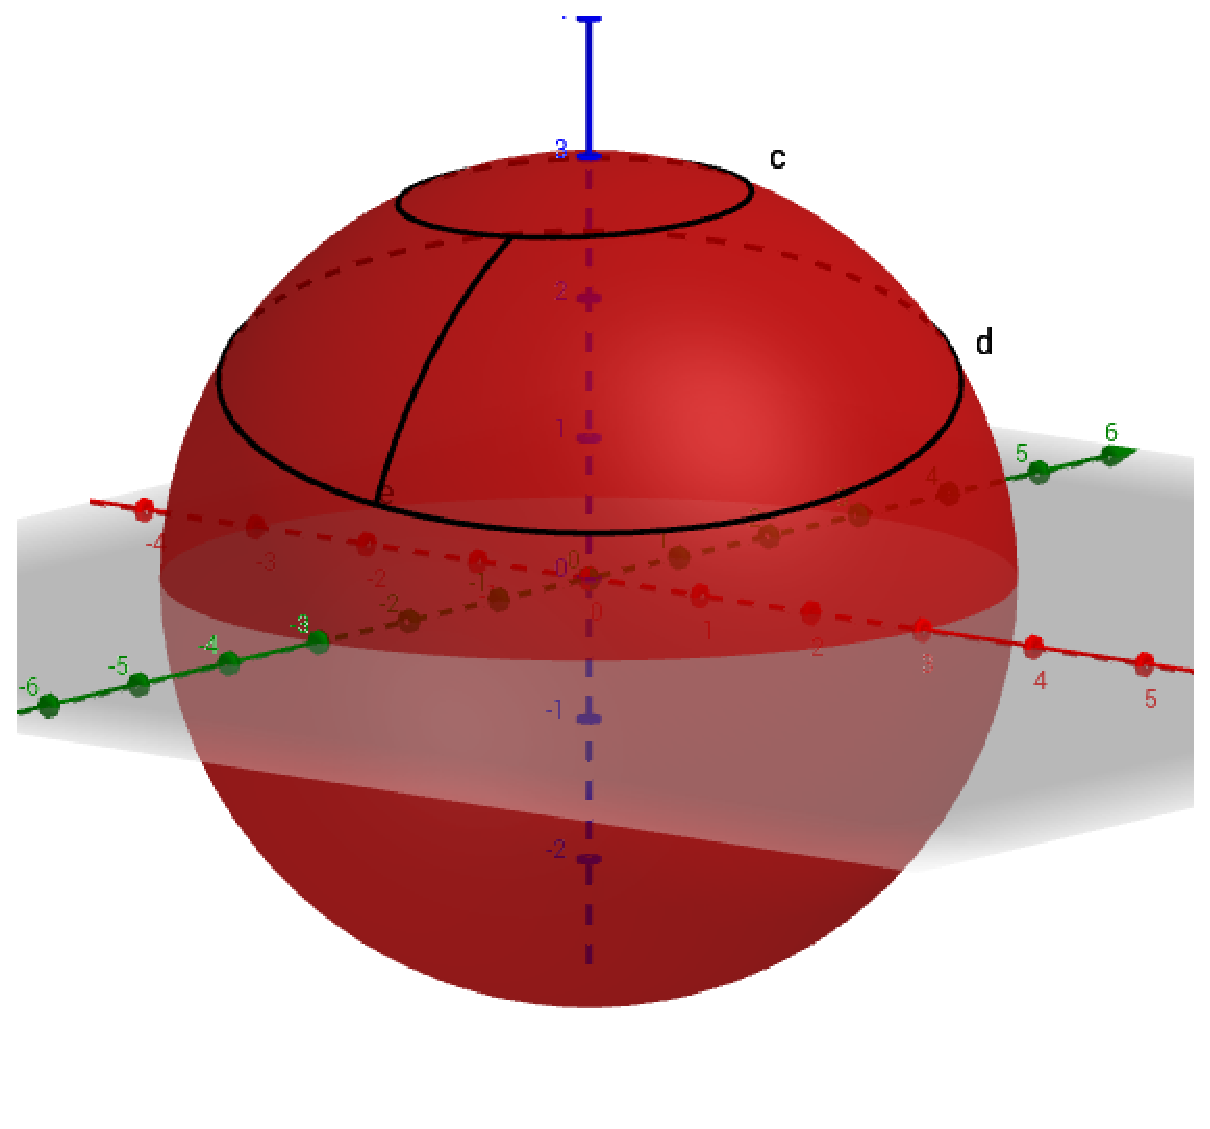
\includegraphics[scale=0.35]{Figures/EsferaParDEspais.eps}
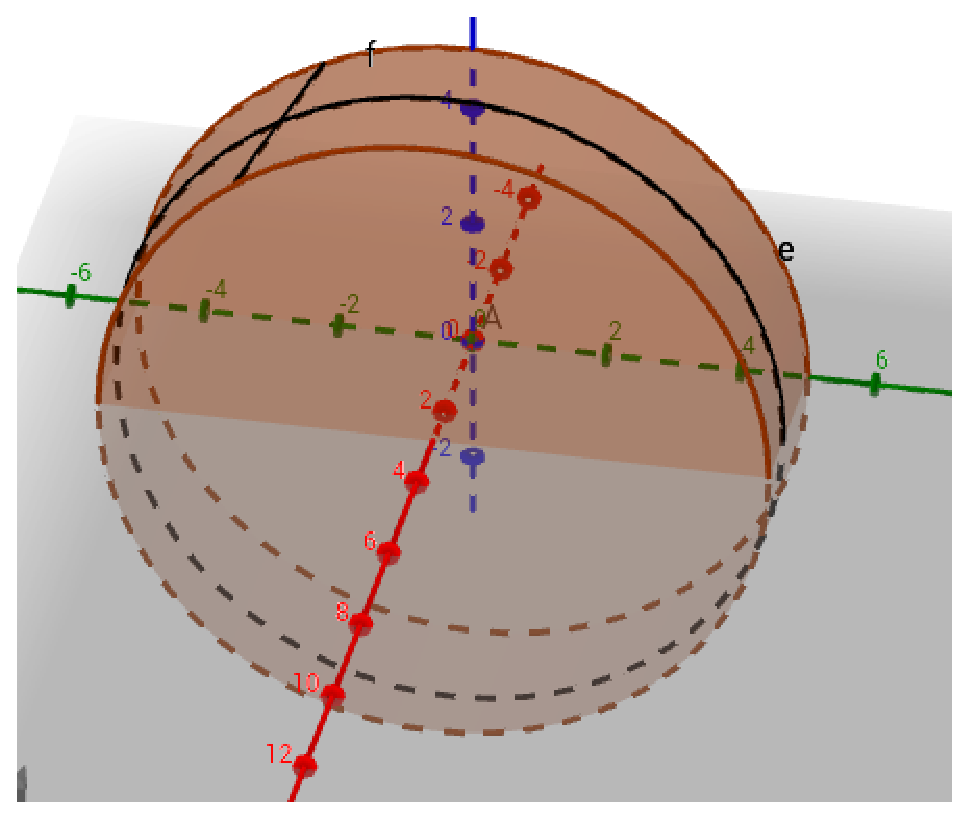
\includegraphics[scale=0.35]{Figures/CilParDEspais.eps}
\caption{\label{FigEsfera} Esfera del ejemplo \ref{EjEsfera} y cilindro de ejemplo \ref{EjCilindro}.}
\end{figure}

\begin{ejem}\label{EjCilindro}
Sea $X$ el cilindro con tapas mostrado en la figura \ref{FigEsfera}, y $A$ la unión de las dos tapas. Sobre $X$ dibujamos la circunferencia $e$ paralela a las anillas del cilindro y el segmento $f$, ambos mostrados en la figura \ref{FigEsfera}.
\\

Por un lado, la curva $e$ es un ciclo en $X$ por ser un lazo, y también lo es en $(X,A)$. Por otro lado, el segmento $f$ no es un ciclo en $X$, pero sí lo es en $(X,A)$. Observar que ambos extremos del camino $f$ recaen en algún punto de $A$.
\end{ejem}

\cuadro{Sea $(X,A)$ un par de espacios. Tomando $C=S_*(X)$ y $D=S_*(A)$ en la sucesión exacta (\ref{SECociente}), se obtiene la \textbf{sucesión exacta asociada al par $(X,A)$}: \ecua{\label{SEPares}H_n(A) \xrightarrow{i_*} H_n(X)\xrightarrow{\pi_*}H_n(X,A)\xrightarrow{\Delta}H_{n-1}(A)}}

\begin{prop}
$i_*$ es un isomorfismo si y sólo si $H_n(X,A)=0$ para todo $n \geq 0$.
\end{prop}

\cuadro{Una \textbf{tríada de espacios} es una terna $(X,A,B)$, donde $(X,A)$ y $(A,B)$ son pares de espacios.}

Sea $(X,A,B)$ una tríada de espacios. Tomando $D=S_*(A)$, $E=S_*(B)$ y $C=S_*(X)$ en (\ref{SECociente2}), se obtiene la sucesión exacta larga $$H_n(A,B) \stackrel{i_*}{\longrightarrow} H_n(X,B) \stackrel{j_*}\longrightarrow H_n(X,A) \stackrel{\Delta'}{\longrightarrow} H_{n-1}(A,B)$$ donde $i_*$ y $j_*$ son los homomorfismos inducidos en homología por las inclusiones $$i: S_*(A) \hookrightarrow S_*(X); \quad j: S_*(B) \hookrightarrow S_*(A)$$ y $\Delta'$ es la aplicación (\ref{DeltaCPrima}).
\\

Recordemos que el grupo libre generado por el vacío es el grupo trivial, de forma que $S_*(\emptyset)=0$. Esto nos permite establecer un isomorfismo natural entre $S_*(X)$ y $S_*(X,\emptyset)$: $$\funcio{f_n}{S_n(X)}{S_n(X,\emptyset)}{c}{c+S_n(\emptyset)}$$ De la misma forma, se tiene que $S_*(X,A,\emptyset) \cong S_*(X,A)$ y $S_*(X)\cong S_*(X,\emptyset,\emptyset)$.

\section{Aplicaciones entre pares}
\cuadro{Sean $(X,A)$ e $(Y,B)$ dos pares de espacios topológicos. Una \textbf{aplicación de pares} $$f: (X,A) \longrightarrow (Y,B)$$ es una aplicación continua $f: X \longrightarrow Y$ tal que $f(A) \subseteq B$.}

Si $\phi: \sigma_p \longrightarrow X$ es un símplice singular tal que $\phi(\sigma_p) \subset A$ y $$f: (X,A) \longrightarrow (Y,B)$$ es una aplicación de pares, se tiene que $(f\circ\phi)(\sigma_p) \subset B$, por lo que $f_\#(\phi)$ es un $p$-símplice singular de $B$. Dado que la elección de $\phi$ es arbitraria y los $p$-símplices singulares conforman una base de $S_*(A)$, se tiene que $$f_\#(S_*(A)) \subseteq S_*(B)$$ por lo que $f$ induce una aplicación de cadenas
\[\begin{array}{cccc}
f_\#:&S_*(X,A)&\longrightarrow&S_*(Y,B)\\
	 &c+S_*(A)&\longmapsto	 &f(c)+S_*(B)
\end{array}\]
que induce a su vez un homomorfismo entre los grupos de homología relativa,
\[\begin{array}{cccc}
f_*:&H_*(X,A)&\longrightarrow&H_*(Y,B)\\
	 &\la c\ra&\longmapsto	 &\la f(c)\ra
\end{array}\]

\cuadro{Sean $f,g: (X,A) \longrightarrow (Y,B)$ aplicaciones entre pares de espacios. Decimos que \textbf{$f$ es homotópica a $g$} si existe una aplicación entre pares de espacios
$$F: (X\times I, A\times I) \longrightarrow (Y,B)$$
tal que $F_0=f$ y $F_1=g$. Observar que $F$, al ser aplicación de pares, se supone continua y verifica que $F(A\times I) \subset B$.}

\begin{teo}
Si $f,g: (X,A) \longrightarrow (Y,B)$ son homotópicas como aplicaciones de pares, $$f_*=g_*: H_*(X,A) \longrightarrow H_*(Y,B)$$
\end{teo}

Tomando $A=\emptyset=B$, se obtiene el teorema de invarianza homotópica. Por tanto, este resultado es una generalización de dicho teorema.

\begin{proof}
Sean $i_0,i_1: (X,A) \longrightarrow (X\times I,A\times I)$ las aplicaciones
$$i_0(x)=(x,0); \quad i_1(x)=(x,1)$$
Se tiene que $f=F\circ i_0$ y $g=F\circ i_1$. Para probar que $f_*=g_*$, basta con probar que $(i_0)_\#$ e $(i_1)_\#$ son homotópicas como aplicaciones de cadenas. La demostración es análoga al teorema de invarianza homotópica.
\end{proof}

\begin{ejem}
Sean $X=[0,1]$, $Y=S_1 \subset \mbR^2$, $A=\{0,1\}$ y $B=\{(1,0)\}$. Considérense las aplicaciones continuas $f,g: X \longrightarrow Y$ definidas como
$$f(x)=e^{2\pi i x}; \quad g(x)=(1,0)$$
Se tiene que $f$ y $g$ son homotópicas, tomando la aplicación $$\funcio{F}{X\times I}{Y}{(x,t)}{e^{2\pi i x}(1-t)+t}$$ y además $f(A)=g(A)=B$, pero no forman una homotopía de pares entre $(X,A)$ e $(Y,B)$.
\end{ejem}

\subsection{Teorema de escisión}
\begin{lema}[Lema de los cinco]
Sean $A_1,\dots, A_{10}$ grupos abelianos. Considérese el diagrama conmutativo
\[\begin{array}{ccccccccc}
A_1&\longrightarrow&A_3&\longrightarrow&A_5&\longrightarrow&A_7&\longrightarrow&A_9\\
%&&&&&&\\
f_1\downarrow&\circlearrowleft&f_2\downarrow&\circlearrowleft&f_3\downarrow&\circlearrowleft&f_4\downarrow&\circlearrowleft&f_5\downarrow\\
%&&&&&&\\
A_2&\longrightarrow&A_4&\longrightarrow&A_6&\longrightarrow&A_8&\longrightarrow&A_{10}
\end{array}\]
cuyas filas forman sucesiones exactas. Si $f_1$ es un epimorfismo, $f_2$, $f_4$ son isomorfismos y $f_5$ es un monomorfismo, $f_3$ es un isomorfismo.
\end{lema}

\begin{teo}[Teorema de escisión]
Sea $(X,A)$ un par de espacios y $U \subset A$ tal que $\overline{U} \subset \mbox{int}(A)$. Se tiene que la aplicación inclusión \[\funcio{i}{(X-U,A-U)}{(X,A)}{(x,y)}{(x,y)}\] induce un isomorfismo $$i_*: H_*(X-U,A-U) \longrightarrow H_*(X,A)$$
\end{teo}

\begin{figure}[h]
\centering
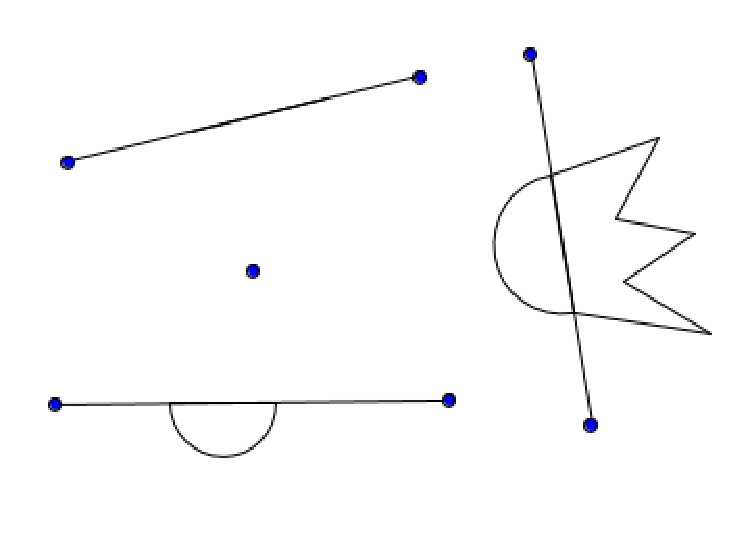
\includegraphics[scale=0.7]{Figures/TeoEsci}
\caption{El teorema de escisión nos dice que da igual qué tipo de figura adjuntemos al punto del centro en tanto que peguemos los dos extremos (resaltados en azul). Todas tendrán la misma homología relativa.}
\end{figure}

\begin{proof}
Sea $\mathcal{U}$ un recubrimiento de $X$ formado por los conjuntos $X-U$ e int$_X(A)$. Se tiene que $$\mbox{int}(X-U)=X-\overline{U} \supset X-\mbox{int}(A)$$ luego $X-U$ e int$(A)$ forman un recubrimiento de $X$. Sea $\mathcal{U}'$ el recubrimiento de $A$ formado por $A-U$ y int$_X(A)$. Por la misma razón, se tiene que int$_A(A-U)$ e int$_X(A)$ también forman un recubrimiento de $A$.
\\

En virtud del teorema 7, sabemos que los homomorfismos $$i: S_*^\mathcal{U}(X) \hookrightarrow S_*(X);\quad i': S_*^{\mathcal{U}'}(A) \hookrightarrow S_*(A)$$ forman isomorfismos entre los grupos de homología. Teniendo en cuenta que $S_*^{\mathcal{U}'}(A) \leq S_*^\mathcal{U}(X)$, la aplicación inclusión $$j: \frac{S_*^\mathcal{U}(X)}{S_*^{\mathcal{U}'}(A)} \hookrightarrow \frac{S_*(X)}{S_*(A)}=S_*(X,A)$$ forma una aplicación de cadenas que da lugar al diagrama conmutativo
\[\begin{array}{ccccccc}
H_n(S_*^{\mathcal{U}'}(A))&\longrightarrow&H_n(S_*^\mathcal{U}(X))&\longrightarrow&H_n\left(\frac{S_*^\mathcal{U}(X)}{S_*^{\mathcal{U}'}(A)}\right)&\longrightarrow&H_{n-1}(S_*^{\mathcal{U}'}(A))\\
%&&&&&&\\
i'_*\downarrow&\circlearrowleft&i_*\downarrow&\circlearrowleft&j_*\downarrow&\circlearrowleft&i'_*\downarrow\\
%&&&&&&&\\
H_n(A)&\longrightarrow&H_n(X)&\longrightarrow&H_n(X,A)&\longrightarrow&H_{n-1}(A)
\end{array}\]

Como $i_*$ e $i'_*$ son isomorfismos, el lema de los cinco nos garantiza que $j_*$ es un isomorfismo. No obstante, no relaciona los espacios que nos interesan. Ahora bien, si $A,B,C$ son grupos abelianos tales que $B+C \leq A+C$, podemos asegurar que $$\frac{A+C}{B+C} \cong \frac{A}{B} \implies S_*(X-U,A-U) \cong \frac{S_*^\mathcal{U}(X)}{S_*^{\mathcal{U}'}(A)}$$

Por tanto,
$$H_*(X,A)\cong H_*\left(\frac{S_*^\mathcal{U}(X)}{S_*^{\mathcal{U}'}(A)}\right) \cong H_*(X-U,A-U)$$
\end{proof}

\begin{ejem}
Sea $X=S^2$, $A$ el área comprendida entre los trópicos de la $S^2$ y $U$ el ecuador. Se tiene que $X-U$ son dos casquetes y $A-U$ son dos bandas. Ahora bien, observar que
$$\frac{X-U}{A-U} \cong \frac{X}{A}$$
por lo que tienen el mismo tipo de homología.

\begin{figure}[h]
\centering
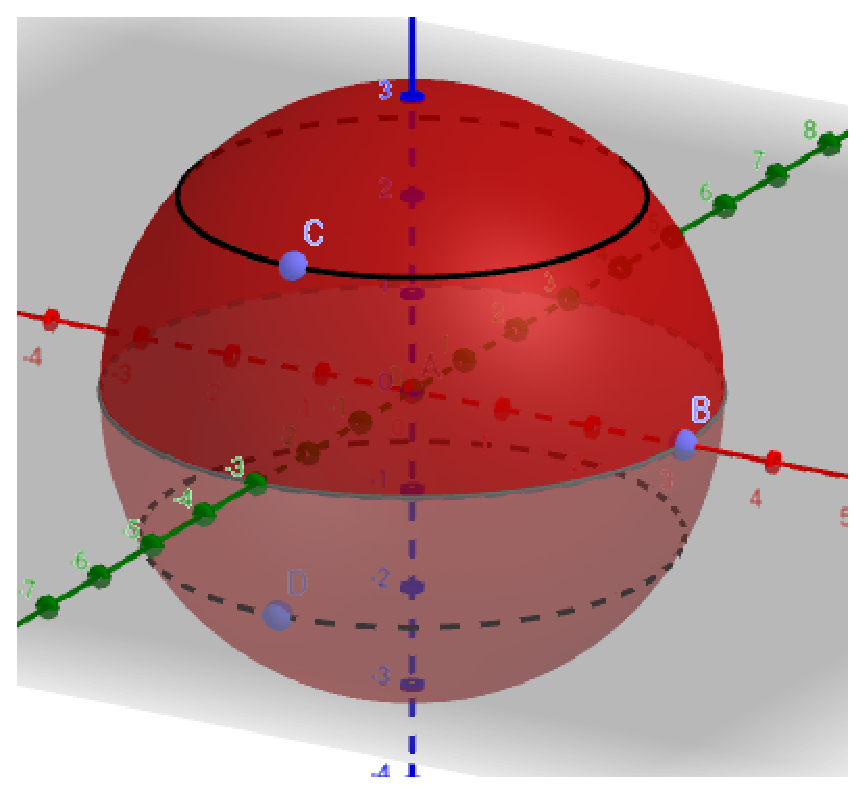
\includegraphics[scale=0.5]{Figures/EsciEsfera.eps}
\caption{Los trópicos son las circunferencias que pasan por los puntos $C$ y $D$.}
\end{figure}
\end{ejem}

\begin{ejem}
Sean $X=[0,1]^2/\sim$ el toro llano, $$A=\frac{[1/4,3/4]\times[0,1]}{\sim} \subset X$$ y $\star$ un subespacio puntual de $A$.
\\

$X-\star$ es un toro perforado. Poedmos tomar el agujero y ensancharlo hasta quedarnos con dos «hilos de alambre» cruzados (que son los generadores de $H_1$). Esos hilos forman una figura ocho.
\\

\begin{figure}[h]
\centering
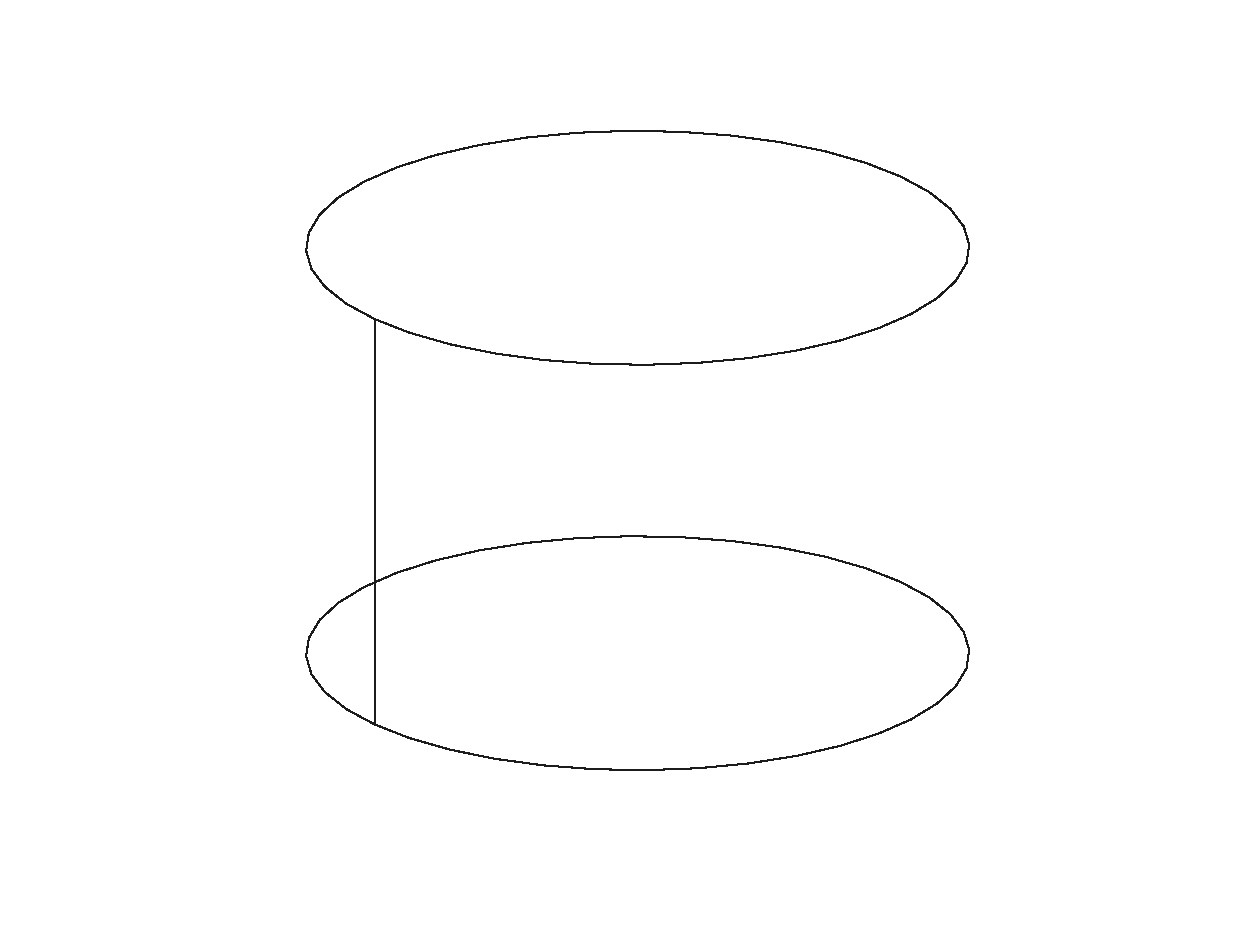
\includegraphics[scale=0.4]{Figures/1EsqCilindro.eps}
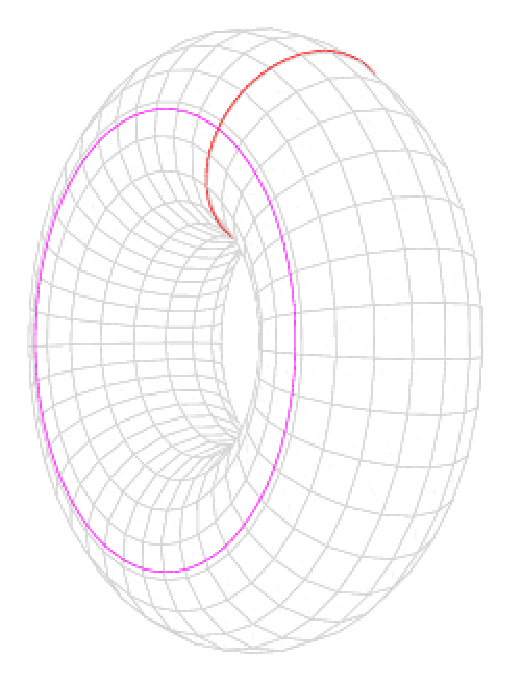
\includegraphics[scale=0.5]{Figures/FiguraOcho.eps}
\caption{Resultado de ensanchar la perforación.}
\end{figure}

Por otro lado, $A-\star$ es un cilindro perforado. Podemos tomar la perforación y ensancharla hasta quedarnos con las anillas de los bordes y un alambre que los une. Dicho alambre se puede retraer hasta que las dos anillas sean tangentes, formando una figura ocho.
\end{ejem}

\section{Grupo de homología reducida}
Sea $X \in \topo$ y $\star$ un espacio puntual. Considérese la curva $\alpha: X \longrightarrow \star$, que es claramente una aplicación constante. $\alpha$ da lugar a un homomorfismo en homologías $\alpha_*: H_*(X) \longrightarrow H_*(\star)$. \cuadro{Se define el \textbf{grupo de homología reducida} como el núcleo de dicho homomorfismo: $$\tilde{H}_*(X):=\ker \alpha_* \leq H_*(X)$$}

Observar que el espacio puntual $X=\{p\}$ es un conjunto convexo, dado que el único segmento que podemos trazar es $[p,p]=\{p\}$. Por tanto, $$\forall i > 0 \quad H_i(X)=0 \implies \tilde{H}_i(X) =0$$ Aún así, no podemos decir nada del grupo de orden 0 porque los singuletes forman espacios arcoconexos, luego $H_0(X)=\mb{Z}$.
\\

La homología reducida está creada para poder describir de forma más sencilla la homología de algunos espacios. Por ejemplo: todos los grupos de homología reducida del espacio puntual son triviales, y el único grupo de homología reducida no trivial de $S^n$ es el de orden $n$, como veremos más adelante.
\\

En general, si un espacio es arcoconexo, su grupo de homología reducida de orden cero es trivial.

\begin{prop}
Sea $X$ un espacio topológico no vacío con una cantidad finita de componentes conexas. $\tilde{H}_0(X)$ es un grupo libre que verifica $$\mbox{rk }(\tilde{H}_0(X))=\mbox{rk }(H_0(X))-1$$
\end{prop}

\begin{proof}
Sea $c$ un $0$-ciclo de $X$. Si llamamos $X_1,\dots,X_n$ a las arcocomponentes de $X$, existirán $a_1,\dots,a_n \in \mb{Z}$ tales que $$c=\sum^n_{i=1}a_ix_i \quad x_i \in X_i \quad (1 \leq i \leq n)$$ Dado que $\alpha$ es una aplicación constante, podemos llamar $\alpha_0$ al valor que toma en todos sus puntos, de forma que $$0=\alpha_*(c+B_0(X))=\sum^n_{i=1}a_i\alpha(x_i)+B_0(X)=\sum^n_{i=1}a_i\alpha_0+B_0(X)$$

De aquí se deduce que $c+B_0(X) \in \ker \alpha_*$ si y sólo si $$a_n=-\sum^{n-1}_{i=1}a_i$$ por lo que $\{x_1,\dots,x_{n-1}\}$ forma un sistema generador libre de $\tilde{H}_0(X)$. Por tanto, $$\tilde{H}_0(X) \cong \mb{Z}^{n-1} \implies \mbox{rk }(\tilde{H}_0(X))=n-1=\mbox{rk }(H_0(X))-1$$ 
\end{proof}

Ahora bien, sea $f: X \longrightarrow Y$ una aplicación continua. Al igual que $f$ induce un homomorfismo entre grupos de homología, queremos ver que $f$ induce un homomorfismo entre grupos de homología reducida. Para ello, sean $\alpha: X \longrightarrow \{p\}$, $\beta: Y \longrightarrow \{p\}$ curvas constantes y $$c=\sum^n_{i=1}a_ix_i: \quad c+B_n(X) \in \tilde{H}_n(X)$$ Se tiene que $$f_*(c+B_n(X))=\sum^n_{i=1}a_if(x_i)=\sum^m_{j=1}b_jy_j$$ Dado que las aplicaciones continuas llevan conjuntos arcoconexos en conjuntos arcoconexos, se tiene que $$\sum^n_{i=1}a_i=\sum^m_{j=1}b_j$$

Si $c+B_n(X)$ está en $\ker \alpha_*$, deberá suceder que la suma de todos los $a_i$ sea 0. Como la suma de los $a_i$ es la misma que la de los $b_j$, esto es tanto como decir que $f_*(c+B_n(X))$ está en $\ker \beta_*$. Por tanto, $f_*(\ker \alpha_*) \leq \ker \beta_*$, de forma que $f$ induce un homomorfismo $$\tilde{f}_*: \tilde{H}_*(X) \longrightarrow \tilde{H}_*(Y)$$ entre los grupos de homología reducida.

\begin{ejem} Si $X$ es un espacio contráctil, $\tilde{H}_*(X)=0$. \end{ejem}

\subsection{Una fórmula para la homología reducida}
\begin{lema}[Lema de escisión]
Sean $A,B,C$ grupos abelianos. Considérese la sucesión exacta corta $$0 \longrightarrow A \xrightarrow{f} B \xrightarrow{g} C \longrightarrow 0$$ Las siguientes afirmaciones son equivalentes:
\lista{
\item $B$ es suma directa de $A$ con $C$.
\item Existe un homomorfismo $h: B \longrightarrow A$ tal que $f\circ h=1_A$.
\item Existe un homomorfismo $k: C \longrightarrow B$ tal que $k\circ g=1_C$.}
\end{lema}

\begin{prop} Dado un $p \in X$, $$\tilde{H}_*(X)\cong H_*(X,\{p\})$$\end{prop}

\begin{proof}
Sea $i: \{p\} \hookrightarrow X$ la inclusión. La aplicación continua $$\alpha: X \longrightarrow {p}$$ verifica que $1_{\{p\}}=\alpha\circ i$, por lo que $\{p\}$ forma un retracto de $X$ e $i_*$ es un monomorfismo.
\\

Considérere la sucesión exacta de homología generada por el par de espacios $(X,\{p\})$: $$H_n(\{p\}) \xrightarrow{i_*} H_n(X) \xrightarrow{j_*} H_n(X,\{p\}) \xrightarrow{\Delta'} H_{n-1}(\{p\})$$ Como $i_*$ es un monomorfismo, $\im \Delta'=\ker i_*=0$. Por el primer teorema de isomorfia, $\im j_*=\ker \Delta'=H_n(X,p)$, por lo que $j_*$ es sobreyectiva.
\\

Dado que $i_*$ es inyectiva y $j_*$ es sobreyectiva, podemos pasar a definir una sucesión exacta corta en lugar de trabajar con una sucesión exacta larga: $$0 \longrightarrow H_n(\{p\}) \xrightarrow{i_*} H_n(X) \xrightarrow{j_*} H_n(X,\{p\}) \longrightarrow 0$$

Sabemos que $\alpha_* \circ i_*=1_{H_*(\{p\})}$, por lo que el lema de escisión nos garantiza que existe un homomorfismo $$\beta: H_n(X,\{p\}) \longrightarrow H_n(X)$$ tal que $j_*\circ \beta=1_{H_n(X,\{p\})}$. Esto es tanto como decir que $\beta$ es inyectiva.
\\

Se puede probar que $\im \beta=\ker \alpha_*=\tilde{H}_*(X)$, por lo que hemos hallado un isomorfismo entre $H_*(X,\{p\})$ y $\tilde{H}_*(X)$.
\end{proof}

Sea $X$ un espacio topológico con $n$ componentes arcoconexas. Hasta ahora, sabemos que $$\tilde{H}_0(X) \cong \mb{Z}^{n-1}$$ pero queda pregunta preguntarnos qué ocurre con los grupos de orden superior. Utilizando esta proposición que acabamos de probar, tenemos para cada $p > 0$ y el espacio puntual $\star$ que \[\tilde{H}_p(X)\cong H_p(X,\star)=\frac{Z_p(X,\star)}{B_p(X,\star)}=\frac{Z_p(X)/Z_p(\star)}{B_p(X)/B_p(\star)}\] Teniendo en cuenta que $Z_p(\star)=B_p(\star)$, estamos en condiciones de aplicar el tercer teorema de isomorfia: \[\tilde{H}_p(X)\cong \frac{Z_p(X)/Z_p(\star)}{B_p(X)/B_p(\star)}=\frac{Z_p(X)/B_p(\star)}{B_p(X)/B_p(\star)} \cong \frac{Z_p(X)}{B_p(X)}=H_p(X)\]

De esta forma, llegamos a que el grupo de homología reducida sólo \textit{reduce} el grupo de orden cero, cuya única función es contar el número de componentes conexas.

\begin{cor}
\cuadro{Sea $X$ un espacio topológico con una cantidad finita de arcocomponentes. \[\tilde{H}_*(X)\cong \frac{H_*(X)}{H_*(\star)}\]}
\end{cor}

\begin{ejem}
$$\tilde{H}_*(B_p)\cong\frac{H_*(B_p)}{H_*(\star)}\cong\begin{cases}\mb{Z}^p & \mbox{ si } n=1\\0 & \mbox{ si no}\end{cases}$$
\end{ejem}

\subsection{Homología reducida y homología relativa}
En lo sucesivo, diremos que un espacio topológico es de \textbf{tipo $C_2$} si es compacto y $T_2$ al mismo tiempo.

\begin{lema}\label{RetrCoci}
Sea $(X,A)$ un par de espacios donde $X$ es $C_2$ y $A$ es cerrado $X$. Considérese la aplicación cociente $$\pi: X \longrightarrow \frac{X}{A}$$ y sea $y=\pi(A) \in X/A$. Si $A$ es retracto por deformación fuerte de $X$, $\{y\}$ es un retracto por deformación fuerte de $\pi(X)=X/A$.
\end{lema}

\begin{nota}
Sea $X$ un espacio topológico, $\sim$ una relación de equivalencia sobre $X$ y $$\pi: X \longrightarrow X/\sim$$ una proyección.
\\

Todo punto $v \in X/\sim$ es una clase de equivalencia de $X$, y $\pi^{-1}(v)$ es el conjunto de todos sus posibles representantes.
\end{nota}

\begin{proof}
Dado que $A$ es un retracto por deformación fuerte de $X$, existe una homotopía $F: X \times I \longrightarrow X$ tal que $F_0=1_X$, $(F_t)|_A=1_A$ y $F_1(X) \subseteq A$.
\\

Si $X_A=X/A$, queremos hallar una homotopía $G: X_A\times I \longrightarrow X_A$ tal que $G_0=1_{X/A}$, $G_1(X_A,t)=\{y\}$ y $G(y,t)=y$ para todo $t \in I$. En el lema, nos proporcionan una aplicación cociente $\pi$ que envía $X$ en $X_A$ de forma continua, por lo que nuestro impulso inicial sería definir $$G=\pi \circ F \circ (\pi \times 1_I)^{-1}$$

El problema está en que $\pi^{-1}$ no está bien definida, por lo que tampoco lo va a estar $(\pi\times 1_I)^{-1}$. Lo que sí es cierto es que, de estar bien definida, la fórmula anterior sería equivalente a $$G\circ  (\pi \times 1_I)=\pi \circ F$$ Este razonamiento nos invita a definir la aplicación $$\funcio{G}{X_A\times I}{X_A}{([x]_A,t)}{(\pi \circ F)(x,t)}$$

\noindent\textbf{$G$ está bien definida y $G(y,t)=y$ para todo $t \in I$}
\\
Si $x \not\in A$, la clase de $x$ módulo $A$ es el singulete formado por el propio punto $x$, por lo que $G$ está bien definido en $X_A-\{y\}$.
\\

Por otro lado, si $x \in A$, sabemos que $$F(a,t)=a \quad \forall t \in I \implies (\pi\circ F)(a,t)=\pi(a) \in \pi(A)=\{y\}$$ De esta forma, se tiene que $G$ está bien definida y que $G_t|_A=1_A$ para todo $t \in I$.
\\

\noindent\textbf{$G$ es una deformación ($G_0=1_{X/A}$)}
\\
Sea $p \in X/A$. Si $x \in \pi^{-1}(p)$, sabemos que $F_0(x)=x$, por lo que $$G_0(p)=(\pi\circ F)(x,0)=\pi(x)=p \implies G_0=1_{X/A}$$

\noindent\textbf{$G$ es un retracto ($G_1(X/A)=\{y\}$)}\\
Sea $p \in X/A$ y $x \in \pi^{-1}(p)$. Sabemos que $F_1(x) \in A$, por lo que \[G(p,1)=(\pi \circ F)(x,1)\in \pi(A)=\{y\} \implies G(X_A,1)\subseteq\{y\}\]

\noindent\textbf{$G$ es continua}\\
Para ver que $G$ es continua, comprobaremos que la antiimagen de cualquier cerrado es cerrado.
\\

Sea $C$ un subconjunto cerrado de $X/A$. $F$ y $\pi$ son aplicaciones continuas, por lo que $D=(\pi\circ F)^{-1}(C)$ es un subconjunto cerrado de $X\times I$. Como $X\times I$ es compacto y todo subconjunto cerrado de un compacto hereda la compacidad, $D$ es compacto.
\\

$\pi$ y $1_I$ son aplicaciones continuas, por lo que $(\pi\times 1_I)(D)$ es compacto. Por cómo se define $G$, se tiene que $G^{-1}(C)=(\pi\times 1_I)(D) \subseteq X_A \times I$. Dado que $X_A\times I$ es un espacio de Hausdorff y $G^{-1}(C)$ es compacto, es cerrado.
\\

Dado que la elección de $C$ es arbitraria, se sigue que $G$ es continua.\end{proof}

\begin{lema} Sea $X$ un espacio $C_2$. Dados dos cerrados disjuntos $C,D \subset X$, existen abiertos $U,V \subset X$ tales que $U$ contiene a $C$, $V$ contiene a $D$ y $U\cap V=\emptyset$ \end{lema}

\begin{proof}
Dado un $x \in C$ y un punto $y \in D$, como $C$ y $D$ son disjuntos, $x \neq y$. Como $X$ es $T_2$, existen $U_y, V_y$ abiertos tales que $$x \in U_y \quad\land\quad y \in V_y \quad\land\quad U_y\cap V_y=\emptyset$$ Como $D$ es un subespacio cerrado de un compacto, $D$ es compacto, por lo que podemos hallar una familia finita de puntos $y_1,\dots,y_n \in D$ tales que $\{V_{y_1},\dots, V_{y_n}\}$ es un recubrimiento abierto de $D$.
\\

Para cada $i \in \{1,\dots,n\}$, podemos hallar un abierto $U_i \subseteq X$ tal que $U_i\cap V_{y_i}=\emptyset$ y $x \in U_i$. Se definen entonces $$U_x=\bigcup_{i=1}^nU_i \quad\land\quad V_x=\bigcup_{i=1}^n V_{y_i}$$ Notar que ambos conjuntos son abiertos y $U_x\cap V_x=\emptyset$.
\\

Dado que $C$ es un subespacio cerrado de un compacto, $C$ es compacto, por lo que podemos hallar una familia finita de puntos $x_1,\dots,x_n$ tales que $\{U_{x_1},\dots,U_{x_m}\}$ forma un recubrimiento abierto de $C$.
\\

Para terminar, considérense los abiertos $$U=\bigcup _{i=1}^m U_{x_i} \quad\land\quad V=\bigcup_{i=1}^m V_{x_i}$$ Se tiene que $D \subseteq V$ y $U\cap V=\emptyset$.
\end{proof}

\begin{lema}\label{LemaB} Sea $X$ un espacio $C_2$. Dado un cerrado $A$ contenido en un abierto $V$, existe un abierto $W$ tal que $$A \subseteq W \subseteq \overline{W} \subseteq V$$\end{lema}

\begin{proof}
Considérense los cerrados $A$ y $X-V$. Por el lema anterior, existen abiertos $U,W$ de $X$ tales que $A \subseteq W$, $X-V \subseteq U$ y $U\cap W=\emptyset$. $$U\cap W =\emptyset \implies W \subseteq X-U \subseteq V \implies \overline{W} \subset \overline{X-U}=X-U \subseteq V$$ Observar que $X-U$ es cerrado.\end{proof}

\begin{teo}[Teorema del retracto]
Sea $X$ un espacio $C_2$, $A$ un subespacio cerrado de $X$ y $\pi: (X,A) \longrightarrow (X/A,\pi(A))$ una aplicación cociente. Si $A$ es un retracto por deformación fuerte de algún entorno cerrado de $A$ en $X$, $$H_*(X,A) \cong H_*\left(\frac{X}{A},y\right) \cong \tilde{H}_*\left(\frac{X}{A}\right)$$
\end{teo}

\begin{proof} \textbf{Paso 1:}
\\
Considérese la sucesión exacta asociada a la tríada de espacios $(X,U,A)$: \[H_n(U,A) \xrightarrow{i_*} H_n(X,A) \xrightarrow{j_*} H_n(X,U) \xrightarrow{\Delta'} H_{n-1}(U,A)\] Dado que $A$ es un retracto por deformación fuerte de $U$, se tiene que $H_*(U,A)=0$. Por exactitud, se sigue que $0=\im i_*=\ker j_*$ y $\im j_*=\ker \Delta'=H_n(X,U)$. Por tanto, $$j_*: H_n(X,A) \xrightarrow{\quad\cong\quad} H_n(X,U)$$

\noindent\textbf{Paso 2:}
\\
Sabemos que $X$ es un espacio $C_2$ y que $A$ es cerrado. Como $U$ es entorno de $A$, $A \subseteq \mbox{int}(U)$, que es un abierto. En virtud del lema \ref{LemaB}, podemos hallar un abierto $V \subseteq X$ tal que $$A \subseteq V \subseteq \overline{V} \subseteq \mbox{int}(U) \subseteq U$$

Aplicando el teorema de escisión, se tiene que  la inclusión $$i: (X-V,U-V) \hookrightarrow (X,U)$$ induce un isomorfismo $i_*: H_*(X-V,U-V) \longrightarrow H_*(X,U)$, por lo que $$i_*^{-1}: H_*(X,U) \xrightarrow{\quad\cong\quad} H_*(X-V,U-V)$$

\noindent\textbf{Paso 3:}
\\
Considérese la aplicación $$\funcio{p}{X-V}{X_A-\pi(V)}{x}{\pi(x)}$$ Como $A \subseteq V$, se tiene que $\pi(x)$ sólo tiene un representante (al propio $x$), de forma que $p$ es un homeomorfismo. Como $\pi(U-V)=\pi(U)-\pi(V)$, se sigue que $$p_*: H_*(X-V,U-V) \xrightarrow{\quad\cong\quad} H_*(X_A-\pi(V),\pi(U)-\pi(V))$$

\noindent\textbf{Paso 4:}
\\
De la misma forma que hicimos en el paso 2, podemos aplicar el teorema de escisión al par $(X_A,\pi(U))$, con lo que se obtiene que $$i_*: H_*(X_A-\pi(V),\pi(U)-\pi(V)) \xrightarrow{\quad\cong\quad} H_*(X_A,\pi(U))$$

\noindent\textbf{Paso 5:}
\\
Considérese la sucesión exacta asociada a la tríada de espacios $(X_A,\pi(U),\pi(A))$. Procediendo de la misma forma que en el paso 1, se tiene que $$j_*: H_n(X_A,\pi(A)) \longrightarrow H_n(X_A,\pi(U))$$ es un isomorfismo, por lo que $$j_*^{-1}: H_n(X_A,\pi(U)) \xrightarrow{\quad\cong\quad} H_n(X_A,\pi(A))$$
\end{proof}

\section{Homeomorfismo relativo}
\cuadro{Un \textbf{homeomorfismo relativo} es una aplicación continua entre pares de espacios $f: (X,A) \longrightarrow (Y,B)$ tal que $$f: X-A \longrightarrow Y-B$$ es un homeomorfismo.}

\begin{ejem}Si $\m{N}=(0,0,1) \in S^2$ y $D^2$ denota a la bola unidad de $\mbR^2$, existe un homeomorfismo $$f: D^2-\partial D^2 \longrightarrow S^2-\{\m{N}\}$$ De esta forma, $f$ induce un homeomorfismo relativo entre los pares $(S^2,\{\m{N}\})$ y $(D^2,\partial D^2)$.
\\

Si $C=S^1\times I$ es un cilindro y $\m{S}$, existe un homeomorfismo $$g: S^1\times \mbox{int}(I) \longrightarrow S^2-\{\m{N},\m{S}\}$$ que identifica al cilindro sin anillas con $S^2$\end{ejem}

\begin{teo}[Teorema del homeomorfismo relativo]
Sean $X,Y$ espacios compactos de Hausdorff, $A \subseteq X$ y $B \subseteq Y$ cerrados y $f: (X,A) \longrightarrow (Y,B)$ un homeomorfismo relativo.\\

Si $A$ es retracto por deformación fuerte de algún entorno compacto de $A$ en $X$ y $B$ es retracto por deformación fuerte de algún entorno compacto de $B$ en $Y$, $f_*$ es un isomorfismo.
\end{teo}

\begin{proof}Sean $\pi: X \longrightarrow X/A$ y $\pi': Y \longrightarrow Y/B$ aplicaciones cociente. Se define la aplicación $$\funcio{f'}{X/A}{Y/B}{[x]_A}{\pi'[f(x)]}$$ Es fácil ver que $f'$ está bien definida y es continua, por lo que da lugar al siguiente diagrama conmutativo:
\[\begin{array}{ccccc}
   	&			&f        			&          	&\\
   	&X   		&\longrightarrow		&Y       	&\\
\pi	&\downarrow	&\circlearrowleft	&\downarrow	&\pi'\\
   	&X/A			&\longrightarrow		&Y/B      	&\\
    &          	&f'       			&          	&
\end{array}\]

Dado que $f$ es un homeomorfismo relativo, $f'$ es una biyección entre $X/A$ e $Y/B$. Como ambos son compactos de Hausdorff, $f'$ es un homeomorfismo, por lo que induce un isomorfismo entre $H_*(X/A)$ y $H_*(Y/B)$.
\\

Denotando $X_A=X/A$ e $Y_B=Y/B$, el diagrama conmutativo anterior induce otro diagrama conmutativo,
\[\displaystyle\begin{array}{ccc}
				&f_*        			&          		\\
H_*(X,A)   		&\longrightarrow		&H_*(Y,B)   		\\
\pi_*\downarrow	&\circlearrowleft	&\downarrow\pi'_*\\
H_*\left(X_A,\pi(A)\right)	&\longrightarrow		&H_*\left(Y_B,\pi'(B)\right)\\
          		&f'       			&          			
\end{array}\]
Sabemos por el teorema 9 que $\pi'_*$ y $\pi_*$ son isomorfismos; además, acabamos de probar que $f_*'$ es un isomorfismo. Todo ello nos lleva a que $f_*$ es un isomorfismo.
\end{proof}
